
\clearemptydoublepage
\pagestyle{empty}\thispagestyle{empty}

%\vspace*{\fill}

\section*{Conseils}

\vspace*{-1ex}

\begin{itemize}
  \item Ce livre utilise la version 3 de Scratch. 
Des vidéos sont accessibles depuis la chaîne \emph{Youtube} :

\centerline{
\href{https://www.youtube.com/c/ScratchAuCollege}{youtube.com/ScratchAuCollege}}

Les vidéos utilisent la version 2 de Scratch, il peut y avoir des variations 
d'une version à l'autre, mais les principes généraux restent les mêmes. 
  
  \item Les scripts Scratch solutions et le livre en couleurs sont disponibles :

  \centerline{\href{https://github.com/exo7math/scratch3-exo7}{github.com/exo7math/scratch3-exo7}}

  \item  Pour progresser plus vite vous pouvez alterner un chapitre  d'activités Scratch (partie 1), des énigmes sur ce chapitre (partie 2), des activités sur feuilles (elles sont indépendantes les unes des autres, partie 3) et encore des énigmes (partie 4) ! 
\end{itemize}




\section*{Les auteurs}

\vspace*{-1ex}

Ce livre est issu du mooc \emph{Scratch au collège} proposé par une équipe formée de :
\begin{center}
Arnaud Bodin\\
Loïc Arsicaud\\
Nathalie Bernard\\
François Recher
\end{center}

\medskip 


Les activités Scratch ont été écrites par Arnaud Bodin et validées par l'équipe. 
Merci à Charlotte pour son aide ! 
Les activités débranchées ont été écrites par Arnaud Bodin et relues par Stéphanie Bodin et François Recher. Nous remercions Laurence Le Foll et Raphaël Petit pour leur relecture.

\medskip 

L'idée de faire une feuille sur le thème \og{}diviser pour régner\fg{} fait suite à une discussion avec Martin Quinson sur son \og{}crêpier psycho-rigide\fg{}.
Merci à Éric Wegrzynowski pour son idée d'activité sur la distance de Levenshtein. Enfin, merci à tous les participants du mooc. 

\medskip 

Nous remercions l'équipe du service multimédia de l'université de Lille pour son travail, en particulier Damien Deltombe pour la réalisation des vidéos, Téodorina Tibar pour l'ingénierie pédagogique et Yannick Bonnaz pour le graphisme. Merci à Christian Tellechea pour son extension LaTeX \og{}Scratch3\fg{}.


\medskip 

Ce projet est porté par le site Exo7 et l'IREM de Lille. 
Nous avons bénéficié du soutien de l'université de Lille, de la COMUE Lille Nord de France et d'une bourse Google CS4HS (\emph{Computer Science for High School}).

\medskip 

\begin{center}
\LogoExoSept{1.5}\qquad\qquad
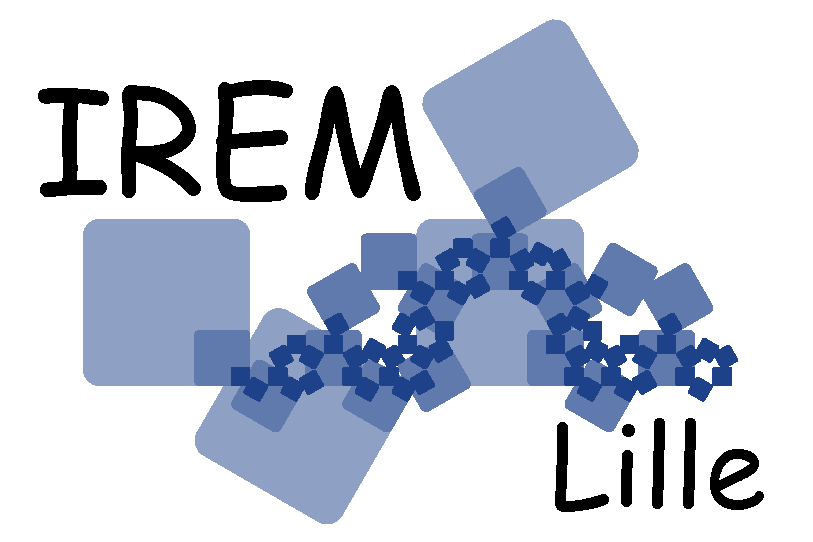
\includegraphics[scale=0.15]{../divers/logo_IREM_de_Lille.pdf}\qquad\qquad
\raisebox{3pt}{
\includegraphics[scale=0.2]{../divers/Logo-Univ-Lille.png}}\qquad\qquad
%\raisebox{3pt}{
\includegraphics[scale=0.16]{../divers/logo-comue.png}}\qquad\qquad
\raisebox{3pt}{
\includegraphics[scale=0.066]{../divers/logo-google.jpg}}
\end{center}



\vspace*{\fill}


\begin{center}
Ce livre est diffusé sous la licence \emph{Creative Commons -- BY-NC-SA -- 4.0 FR}.


% Sur le site Exo7 vous pouvez télécharger gratuitement le livre en couleur\\
% et aussi récupérer les fichiers sources.
\end{center}




%\pagenumbering{gobble} % remove page numbering 
%\printindex
%\pagenumbering{arabic}

